\section{Introduction}

Fact-learning is a well-defined task connected with user modelling.
We focus on a specific subtask of fact-learning, learning of a foreign vocabulary, and aim to provide improvements by modifying the presentation of stimuli during learning.
For this, we consider two new settings: (1) stimulus colour background based on its estimated difficulty by the system and (2) stimulus colour background random (but fixed through the experiment).
The rationale for these two choices is the inutition that the color cues would help in better and faster retrieval of the fact.
Results could lead to faster learning and these improvements could easily be applied to most of commercially available solutions.

% In detail, this means that prior to the study process a colour palette will be selected for every participant. This colour palette associates a different colour to different degrees of difficulty (refer to the next sections for the method to select this colour palette). Each time a word is displayed, the background changes to the colour from the colour palette that represents the difficulty the user model estimates the user is currently having with the word in question.

In a small-scale experiment with learning English translations of Swahili words we aim to answer the following questions (with the accompanying hypotheses):

\begin{itemize}[noitemsep]
\item Does difficulty feedback work better than not providing any extra cues? {$H^1$: Yes.}
\item Does difficulty feedback work better than the random mapping of colours? {$H^2$: Yes.}
\item Do the participants become too reliant on the hints, making it impractical in real-life usage? {$H^3$: No.}
\end{itemize}

The first question is motivated by direct industry application and based on the results, designers of fact-learning apps can be guided in whether to invest in this approach.
Similarly, the second question further refines whether the potential gain is from informing the user of the difficulty or by simply providing an extra-modal content-independent hint.
Finally, the last question provides an insight into whether the users learned to rely on these hints too much, making the approach ineffective in actual learning.

The code for this experiment together with the collected data and participant instructions is open source.\footnote{\href{https://github.com/zouharvi/user-models/}{github.com/zouharvi/user-models}}

\subsection{Related Work}

It has been shown \cite{van2019effects} that providing hints during learning does not have a long-lasting effect on later recall during testing when the hints were not present.
A key difference is, however, that the hints used in their study were relevant to the stimulus, e.g. translating \emph{vestis - clothes: Think of the word ,,vest''}.
Additionally, the hints were shown after the user response for a second chance, forcing the user to work with them and rely on them more closely.
In the case of our experiment, these ,,stimulus content-independent hints'' are shown before the stimulus is answered.
In an extreme case, this may lead to even worse later recall results because the user could associate the answer with the specific colour (see evaluation) and not with the actual stimulus.

The decision to use colours for stimuli-independent cues is motivated by previous work \cite{chang2018impact} which concludes that colours do help with learning and that they work subconsciously on emotions and outside the standard cognitive capacity.
This is in line with the intuition and popular usage of colours in e.g. road signs or visual design.

\section{Setup}

For the experiment interface implementation, we make use of OpenSesame \cite{mathot2012opensesame}.
The modelling of difficulties and selection of stimuli is done by the SlimStampen \cite{sense2016individual} spacing algorithm which also provides the alpha value (rate of forgetting).
This value is an estimate of how difficult it is for the user to recall a specific fact.

\subsection{Experiment}

\subsubsection{Conditions}

We consider the following conditions which we assign to each participant prior to the test (between-subject design):

\begin{itemize}[noitemsep]
\item \textbf{Control group}: always white background
\item \textbf{Difficulty group}: background color based on estimated difficulty
\item \textbf{Random group}: background colour of the word random and constant through the experiment
\end{itemize}

Users were shown a Swahili word to which they were asked to type the English translation.
The English translation was provided for the first time the word was presented and users received feedback after their every response.
\Cref{fig:interface} shows an example of a word and how it is shown under different conditions and difficulty estimates.

\begin{figure}[ht]
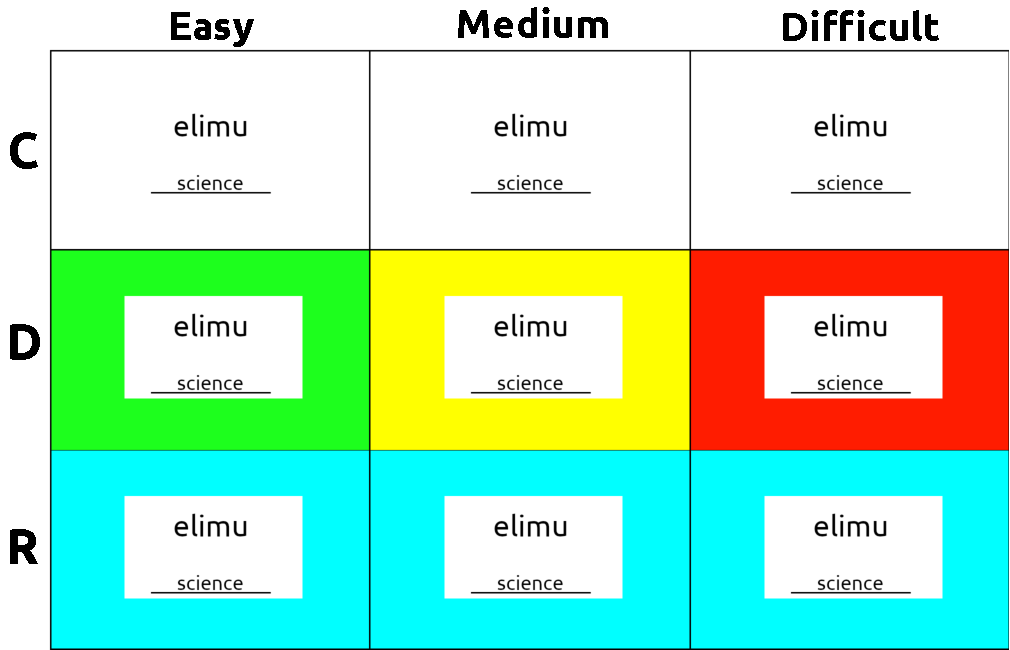
\includegraphics[width=\linewidth]{img/interface.pdf}
\caption{Examples of interfaces in different conditions (C - control, D - difficulty, R - random) and in different difficulty estimates (by alpha value).}
\label{fig:interface}
\end{figure}

\subsubsection{Time overview}

The experiment was split into three main phases: learning phase, distractor and testing phase.
The testing phase was split into two parts.
In the first one, all participants were tasked to provide translations of Swahili words which were shown with white background.
In the second one, the participants saw the words with the colour background in the same condition as for the learning phase.
Participants in the difficulty condition saw colours corresponding to the last difficulty estimate, while participants in the control group saw again only white background.
Responses regarding the correctness of participant answers were not provided during testing and both testing phases independently shuffled the words.
\Cref{tab:progression} shows the time overview of the experiment.
For the learning phase and the distractor phase we strictly controlled the time the participants spent performing the task.

\begin{table}[ht]
\centering
\begin{tabular}{lcc}
\toprule
Event & Duration & Control. Time\\
\midrule
\hspace{0.15cm}Questionnaire 1 & 4 min & No \\
% \cmidrule{1-1}
*Learning Phase & 15 min & Yes \\
*Distractor (Sudoku) & 5 min & Yes \\
*Testing Phase Without Cues & 2-3 min & No \\
*Testing Phase With Cues & 2-3 min & No \\
% \cmidrule{1-1}
*Questionnaire 2 & 3 min & No \\
\bottomrule
\end{tabular}
\caption{Time schedule of the experiment. On-site events/actions marked with *.}
\label{tab:progression}
\end{table}

\subsubsection{Participants}

We enlisted in total 8 male and 9 female masters students of Groningen University of an average age of 24 years.
9 students were Dutch native speakers and others European, North American or Chinese nationals.
None of the participants had any prior knowledge of Swahili.

\subsection{Data}

We use 100 Swahili words and their translations into English used in a prior experiment by \cite{nelson1994norms}.
These are words from not any specific area but rather standard basic vocabulary entries which new students of the language may wish to acquire.
We list 10 examples in the form Swahili - English:
\emph{mbwa - dog, lulu - pearl, wingu - cloud, iktisadi - economy, goti - knee, yai - egg, pombe - beer, godoro - mattress, fagio - broom, tabibu - doctor}.

\subsubsection{Cold Start}

Because the \emph{difficulty} setting is very sensitive to the alpha values which change only slowly over time, we were very particular about the issue of cold start (also known as the ramp-up problem \cite{konstan1998borchers}) and alleviated that using priors from another experiment \cite{nelson1994norms} which we further modified by the following formula.
\textsc{Test-Acc} is the test accuracy of the previous experiment.
$$
0.75 \cdot 0.3 + 0.25 \cdot x + 0.03, x = \frac{\textsc{Test-Acc} - \min X}{\max X - \min X}
$$
This formula is a convex combination of the standard SlimStampen prior of $0.3$ with the weight of $0.75$ and a variable from a previous experiment \cite{nelson1994norms} which was the average test recall accuracy.
Naturally, this variable needs to be transformed into the range $[0,1]$ which we do using a simple min-max scaling.
A constant is added to shift the distribution to the right so that the mean is again $0.3$.
\Cref{fig:cold_start} shows the old data and new data distributions of alpha value estimates.

\begin{figure}[ht]
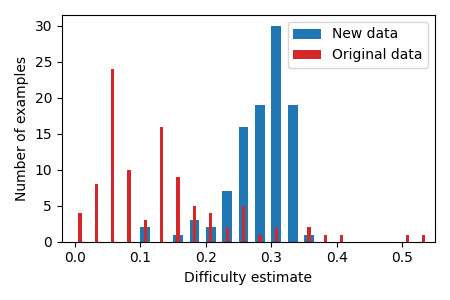
\includegraphics[width=\linewidth]{img/cold_start.png}
\caption{Distribution of alpha value estimates of words (used as priors) based on a previous experiment.}
\label{fig:cold_start}
\end{figure}

\subsubsection{Palettes}

It does not seem to be universal across individuals what colour scale best describes the progression from easy to more difficult.
This was confirmed by a survey with 67 respondents, out of which only 61.2\% chose that their preferred palette is green-white-red.
\Cref{fig:palettes} shows the four palettes which were given to the participants for selection at the beginning of the experiment (if they were part of the difficulty group).

\begin{figure}[ht]
\centering
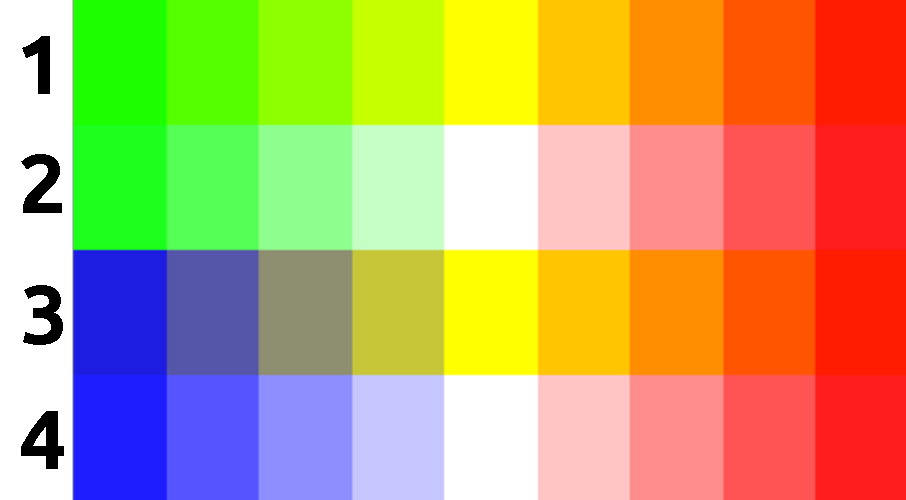
\includegraphics[width=0.6\linewidth]{img/palettes_all.pdf}
\caption{Possible palettes for participants of \emph{difficulty} condition. Each palette starts with easy (left) and progresses to hard (right).}
\label{fig:palettes}
\vspace{-0.1cm}
\end{figure}

The colour palettes were split each into 9 buckets to provide more experiment control.
The palettes are a combination of the initial colour (green or red) and the middle colour (yellow or white), creating 4 configurations in total.
The palette colours were mapped to alpha values from 0.1 (leftmost colour) to 0.5 (rightmost colour).
This was done because rarely do the values exceed this range and we wanted to present the users with the whole spectrum and e.g. not only shades of green.
In case they did, they would be clamped to the colours on the edges.

\section{Results}

We collected results from 17 participants in total with the following distribution per condition:

\vspace{-0.1cm}

\begin{table}[ht]
\centering
\begin{tabular}{lc}
\toprule
Condition & Count \\
\midrule
Control & 5 \\
Difficulty & 7 \\
Random & 5 \\
\bottomrule
\end{tabular}
\end{table}

\vspace{-0.2cm}

\subsection{Testing Phases}

Accuracies of both phases are shown in \Cref{fig:individual_differences}.
Some users did exceptionally well and got 100\% accuracy but there were some which we suspect did not follow the instructions correctly or were not as engaged as required.
We, therefore, filter these two runs out of our analysis (two rightmost users) and for further analysis consider only the rest.
Overall this task exhibits a large degree of individual variance, making drawing statistically significant conclusions difficult.

\begin{figure}[ht]
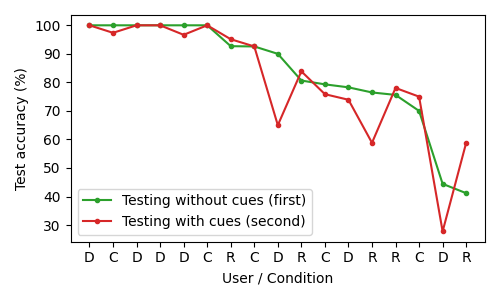
\includegraphics[width=\linewidth]{img/individual_differences.png}
\caption{
    Accuracies in the two testing phases (C - control, D - difficulty, R - random).
    Each point corresponds to one participant (sorted by performance in the first phase).
}
\label{fig:individual_differences}
\end{figure}

We further explore the differences in accuracies in the two testing phases: (1) without colour cues and (2) with colour cues (without cues for the control group).
The results are shown in \Cref{fig:phase_acc}.


\begin{figure}[ht]
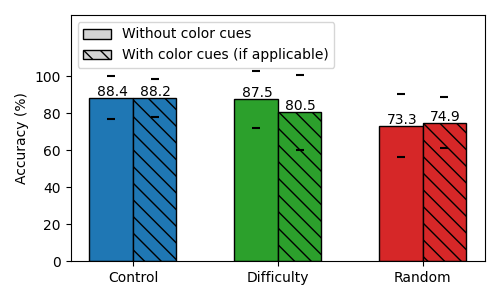
\includegraphics[width=\linewidth]{img/phase_acc.png}
\caption{
    Average accuracies in the two testing phases in different conditions.
    Black horizontal bars denote confidence intervals with 95\% confidence.
}
\label{fig:phase_acc}
\end{figure}

Interestingly, providing the same stimuli to the user did not have a large impact on the performance.
We confirmed this with Kolmogorov–Smirnov test \cite{massey1951kolmogorov} for sameness of distribution with $p<0.05$ for all distributions (highest for the difficulty group).
One explanation would be fatigue or boredom because the users were being tested with the cues always after the testing without cues.
If the results were replicated on a larger sample and with the two phases being ordered randomly, then we could conclude that participants do not become over-reliant on stimuli-independent hints.
This is in contrast to the conclusions for stimuli-dependent hints \cite{van2019effects}.

Unfortunately, it is impossible to determine the usefulness of the two methods (difficulty and random group) because of the low sample size and large individual variance.
At the first glance, the results suggest (without statistical significance), that the provision of random colours associated with words may be distracting and lead to the worsening of accuracy.
The following section discusses why that may not be an issue.

\subsection{Learned Words}

For some learners, the ultimate goal which they try to optimize is not the proportion of correctly answered words to the total number of words (accuracy) but the absolute value of learned words.
For example, in some situations, it may be preferred to learn 200 out of 300 (total exposed) Swahili words (67\% accuracy) over 90 of 100 (total exposed) Swahili words (90\% accuracy).

The selection of facts is done by SlimStampen.
At every step, either an existing fact is selected to force the user to retrieve it from memory or a new one is selected if all existing ones have activations above a certain threshold.
This way, a participant who is consistently getting a fact wrong may encounter fewer facts in the span of 15 minutes than a participant who does better.
We define a word as \emph{encountered} if it has been presented to the participant in the learning phase.
We define a word as \emph{learned} when the participant answers it correctly in both testing phases.
\Cref{fig:learned_words} shows these two quantities per condition.

\begin{figure}[ht]
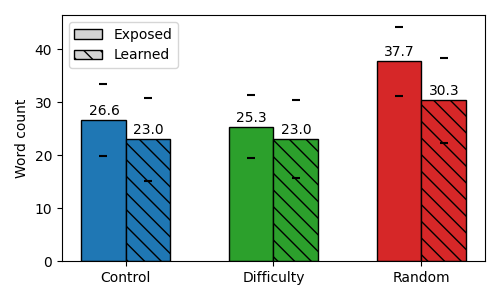
\includegraphics[width=\linewidth]{img/learned_words.png}
\caption{
    Average number of exposed and learned words per participant for every condition.
    Black horizontal bars denote confidence intervals with 95\% confidence.
}
\label{fig:learned_words}
\end{figure}

In contrast to the previous section where the random group had the lowest accuracy, it performs the best from the perspective of learned words (without statistical significance).

\subsection{Questionnaire}

Before and after the in-presence experiment, we solicited information about the participants.
The first questionnaire was centred around biographical and language knowledge information while the latter inquired about participants' participation in the task (self-assessment).  
Although not the primary goal of this project, we found the following.

The average guessed accuracy for the first and the second testing phases was 66.2\% and 72.3\% respectively.
This is less than the actual recorded accuracies.
It also shows that participants were convinced that they did better in the second phase, which was not systematically true.

Participants also reported trying utilizing the colours as a mnemonic, e.g. \emph{cheese = yellow}, shifting towards stimulus-dependency and possibly making it harder to retrieve without this hint.

\section{Conclusion}

We conducted a small-scale experiment with learning Swahili words with stimuli-independent cues.
% Q1
% Q2
Due to the large individual variability, we are not able to soundly conclude whether providing cues based on estimated difficulty or by random colour mappings help more than not providing anything.
The results however suggest that especially the later condition could eventually become a viable option.
% Q3
Attention should be paid to not accidentally provide a colour that matches too well with the word, creating semantic stimulus dependency.
Interestingly, we found no statistical difference ($p<0.05$ for all distributions) when the participants were tested with or without the same colour hints as they learned the words with.

Our current recommendation is not to rely on the intuition that providing these cues must lead to an improvement and test the specific scenario with large enough number of participants.
Duplicating the samples 10 times yielded statistically significant results in line with what we hypotesized.

\subsection{Limitations}

The learning phase itself was very short and making it multi-stage or longer could lead to a more reliable source of data.
Making the distracting phase longer, such as a week instead of 5 minutes, would introduce more noise but would copy a real-life scenario more closely.

To get statistically significant results more participants should be tested.
This could be done using an A/B testing in a commercially deployed application, simulating a less-controlled though on a much larger scale.

\subsection{Future work}

The transition from reliance on stimuli-dependent hints could be done gradually by e.g. making the colours more and more transparent with each successful repetition (or similar technique with textual hints).
It would also be possible to re-use the current setup and analyze other user behaviour properties, such as changes over time.